\lab{Newton's Method, Julia Sets and Basins of Attraction}{Newton's Method}
\label{lab:NewtonsMethod}
\objective{Understand Newton's Method. Understand definition of basin of attraction.  Basic understanding of Julia Sets.}

Newton's method finds the zeros of functions; i.e., Newton's method finds $\overline{x}$ such that $f\left(\overline{x}\right) = 0$.
This method is used to optimize functions (find their maxima and minima), for example to find the zeros of the first derivative.

\section*{Newton's method}
Newton's method begins with an initial guess $x_0$. 
Then recursively define a sequence by
\[
x_{n+1} = x_n - \frac{f(x_n)}{f'(x_n)}
\]
In other words, Newton's method approximates a function by its tangent line, and then uses the zero of the tangent line as the next guess for $x_n$ (see Figure \ref{fig:newton}).

The sequence $\{x_n\}$ will converge to the zero $\overline{x}$ if
\begin{enumerate}
\item $f$, $f'$, and $f''$ exist and are continuous,
\item $f'(\overline{x})\neq0$, and
\item $\overline{x}$ is ``sufficiently close'' to $x_0$.
\end{enumerate}
In applications, the first two conditions usually hold.
However, if $\overline{x}$ and $x_0$ are not ``sufficiently close'', Newton's method may converge very slowly, or it may not converge at all.

\begin{figure}[h]
\centering
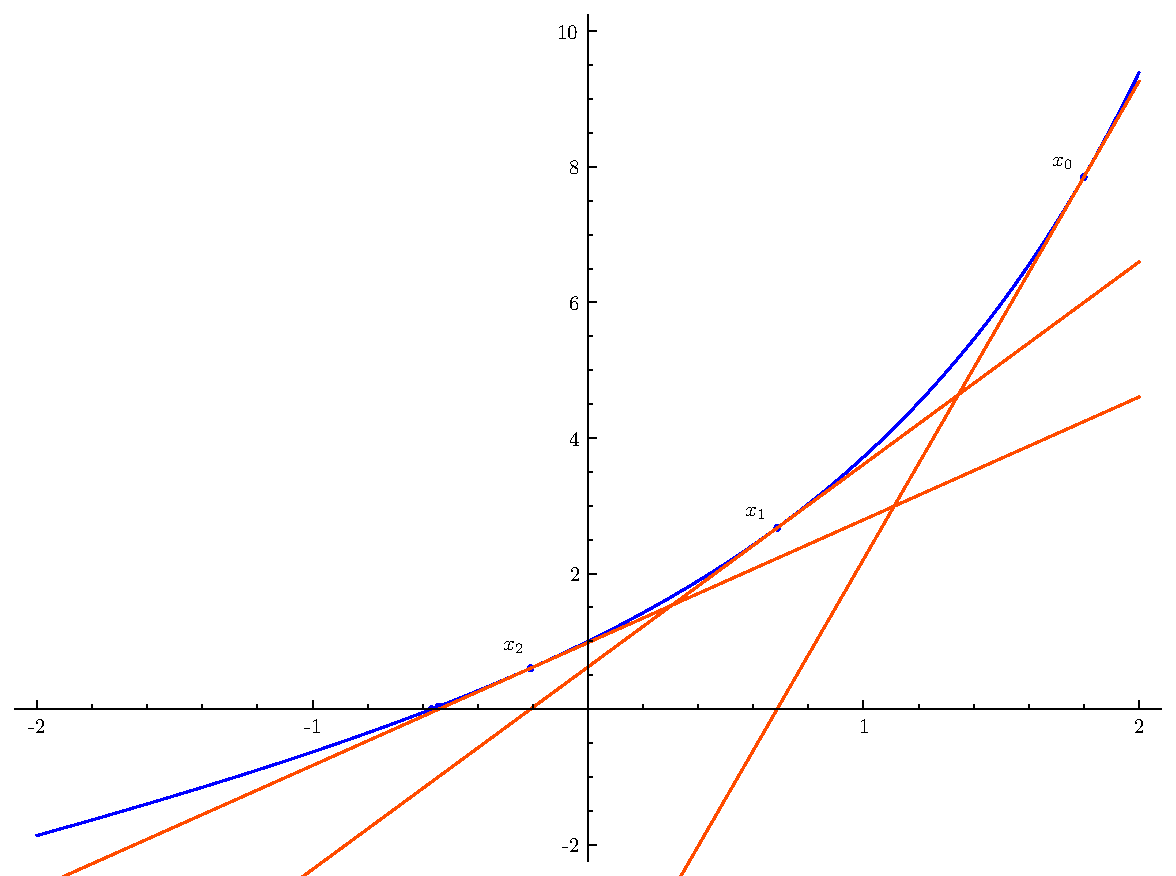
\includegraphics[width=\textwidth]{newton_iters}
\label{fig:newton}
\caption{An illustration of how one iteration of Newton's method works}
\end{figure}

Newton's method is powerful because given the three conditions above, it converges quickly.
In these cases, the $\{x_n\}$ converge to the actual root quadratically, meaning that the maximum error is squared at every iteration.

Let us do an example with $f(x) = x^2-1$. 
We define $f(x)$ and $f'(x)$ in Python as follows. 
\begin{lstlisting}
>>> import numpy as np
>>> from matplotlib import pyplot as plt
>>> f = lambda x : x**2 - 1
>>> Df = lambda x : 2*x
\end{lstlisting}
Now we set $x_0 = 1.5$ and iterate.
\begin{lstlisting}
>>> xold = 1.5
>>> xnew = xold - f(xold)/Df(xold)
>>> xnew
1.0833333333333333
\end{lstlisting}
We can repeat this as many times as we desire.
\begin{lstlisting}
>>> xold = xnew
>>> xnew = xold - f(xold)/Df(xold)
>>> xnew
1.0032051282051282
\end{lstlisting}
We have already computed the root 1 to two digits of accuracy.


\begin{problem}
\label{prob:newton_arr}
\leavevmode
\begin{enumerate}
\item Implement Newton's method with the following function.
\begin{lstlisting}
def Newtons_method(f, x0, Df, iters=15, tol=.002):
    '''Use Newton's method to approximate a zero of a function.
    
    INPUTS:
    f     - A function handle. Should represent a function from 
            R to R.
    x0    - Initial guess. Should be a float.
    Df    - A function handle. Should represent the derivative 
            of `f`.
    iters - Maximum number of iterations before the function 
            returns. Defaults to 15.
    tol   - The function returns when the difference between 
            successive approximations is less than `tol`.
    
    RETURN:
    A tuple (x, converged, numiters) with
    x           - the approximation to a zero of `f`
    converged   - a Boolean telling whether Newton's method 
                converged
    numiters    - the number of iterations the method computed
    '''
\end{lstlisting}

\item Run \li{Newtons_method()} on $f=\cos(x)$ with $x_0=1$ and $x_0=2$. 
How many iterations are required to get 5 digits of accuracy?
\item Newton's method can be used to find zeros of functions that are hard to solve for analytically.
Plot $f(x) = \frac{sin(x)}{x}-x$ on $[-4, 4]$. 
Note that this function can be made continuous on this domain by defining $f(0)=1$. 
Use your function \li{Newtons_method()} to compute the zero of this function to 7 digits of accuracy.
\item Run \li{Newtons_method()} on $f(x)=x^9$ with $x_0=1$. 
How many iterations are required to get 1 digit of accuracy? 
What is the reason for this slow convergence?
\item Run \li{Newtons_method()} on $f(x)=x^{1/3}$ with $x_0=.01$. 
What happens and why?
Hint: The command \li{x**(1/3)} will not work when \li{x} is negative. 
Here is one way to define the function $f(x)=x^{1/3}$ in NumPy.
\begin{lstlisting}
f = lambda x: np.sign(x)*np.power(np.abs(x), 1./3)
\end{lstlisting}
\end{enumerate}
\end{problem}

\begin{problem}(Optional)
Modify the function \li{Newtons_method()} in Problem \ref{prob:newton_arr} so that the argument \li{Df} defaults to \li{None}.
If no derivative is passed to the function, use the centered coefficients method of Lab \ref{lab:NumericalDerivatives} to compute the derivative.
\end{problem}

\begin{comment}
\begin{problem}
Extend your Newton's method even further so that it will work on systems of equations.
Suppose that $F: \mathbb{R}^n \rightarrow \mathbb{R}^n $.
The relevant equation is
\[
x_{i+1} = x_i - J^{-1}F(x_i)
\]
Note that you should not calculate the inverse Jacobian.
\li{scipy.linalg.solve(A,b)} gives you the solution $x$ to the equation $Ax=b$.
Use this fact to calculate $J^{-1}F$ from $J$ and $F$.
You should be able to make this function work whether or not the user inputs a Jacobian.
This also means that you will have to use your own \li{jacobian} function.
\end{problem}
\end{comment}


\section*{Basins of attraction: Newton fractals}
When $f(x)$ has many roots, the root that Newton's method converges to depends on the initial guess $x_0$.
For example, the function $f(x)=x^2-1$ has roots at $-1$ and $1$.
If $x_0<0$, then Newton's method coverges to -1; if $x_0>0$ then it converges to 1 (see Figure \ref{fig:basins1}).
We call the regions $(-\infty, 0)$ and $(0, \infty)$ \emph{basins of attraction}.

\begin{figure}
\begin{center}
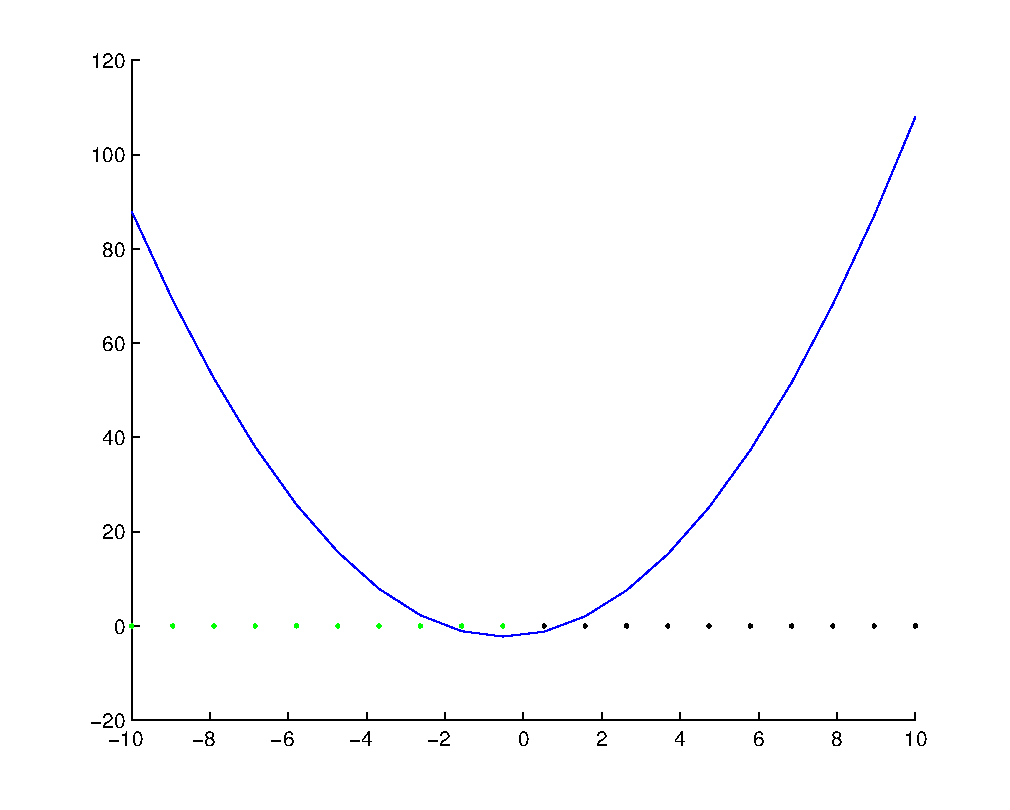
\includegraphics[scale=0.5]{basins1}
\caption{The plot of $f(x) = x^2 -1$ along with some values for $x_0$.
When Newton's method is initialized with a blue value for $x_0$ it converges to -1; when it is initialized with a red value it converges to 1.}
\label{fig:basins1}
\end{center}
\end{figure}

When $f$ is a polynomial of degree greater than 2, the basins of attraction are much more interesting.
For example, if $f(x) = x^3-x$, the basins are depicted in Figure \ref{fig:fractal_1d}.

\begin{figure}
\begin{center}
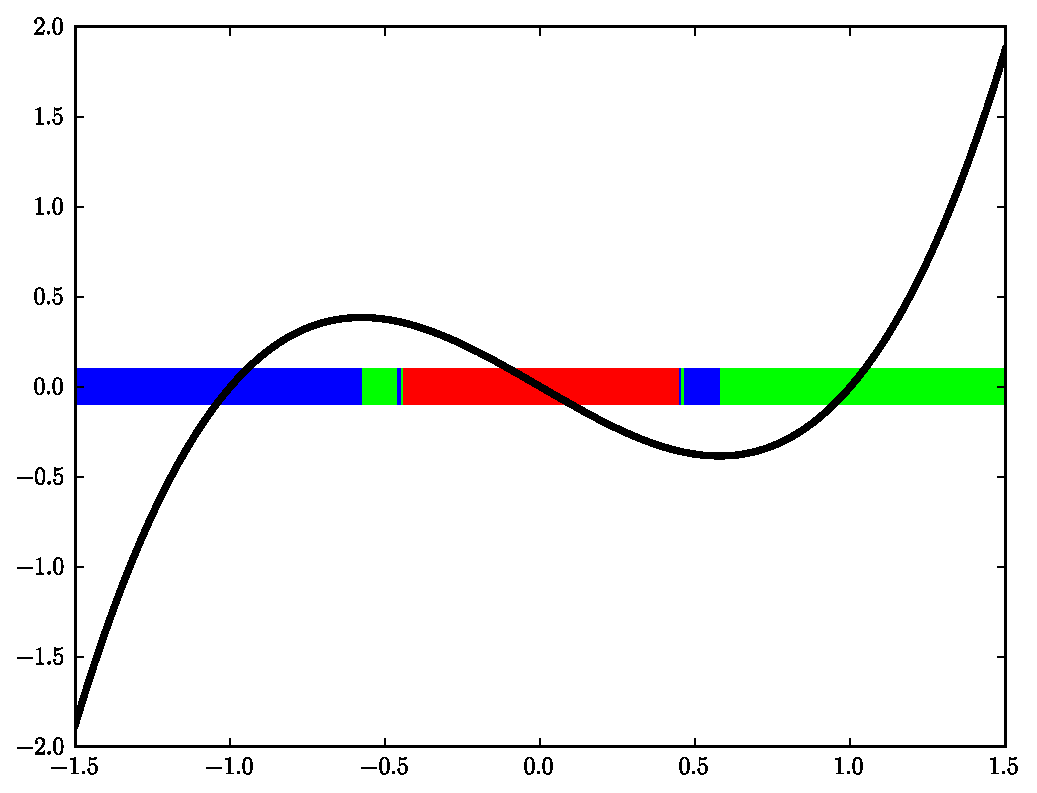
\includegraphics[scale=0.5]{fractal1d}
\caption{The plot of $f(x) = x^3 -x$ along with some values for $x_0$.
Blue values converge to $-1$, red converge to 0, and green converge to 1.}
\label{fig:fractal_1d}
\end{center}
\end{figure}

We can extend these examples to the complex plane. 
Newton's method works in arbitrary Banach spaces with slightly stronger hypotheses (see theorem in textbook), and in particular it holds over $\mathbb{C}$.

Let us plot the basins of attraction for $f(x) = x^3-x$ on the domain $\{a+bi \mid (a, b) \in [-1.5, 1.5] \times [-1.5, 1.5] \}$ in the complex plane.
We begin by creating a $700 \times 700$ grid of points in this domain. 
We create the real and imaginary parts of the points separately, and then use \li{np.meshgrid()} to turn them into a single grid of complex numbers.
\begin{lstlisting}
>>> xreal = np.linspace(-1.5, 1.5, 700)
>>> ximag = np.linspace(-1.5, 1.5, 700)
>>> Xreal, Ximag = np.meshgrid(xreal, ximag)
>>> Xold = Xreal+1j*Ximag
\end{lstlisting}
Recall that \li{1j} is the complex number $i$ in NumPy. 
The array \li{Xold} contains $700^2$ complex points evenly spaced in the domain.

We may now perform Newton's method on the points in \li{Xold}. 
\begin{lstlisting}
>>> f = lambda x : x**3-x
>>> Df = lambda x : 3*x**2 - 1
>>> Xnew = Xold - f(Xold)/Df(Xold)
\end{lstlisting}
After iterating the desired number of times, we have an array \li{Xnew} whose entries are various roots of $x^3-x$.

Finally, we plot the array \li{Xnew}. The result is similar to Figure \ref{fig:fractal_ex}.
\begin{lstlisting}
>>> plt.pcolormesh(Xreal, Ximag, Xnew)
\end{lstlisting}

Notice that in Figure \ref{fig:fractal_ex}, whenever red and blue try to come together, a patch of green appears inbetween.
This behavior repeats on an infinitely small scale, producing a fractal.
Because it arises from Newton's method, this fractal is called a \emph{Newton fractal}.

\begin{figure}
\begin{center}
\begin{subfigure}[b]{.49\textwidth}
\centering
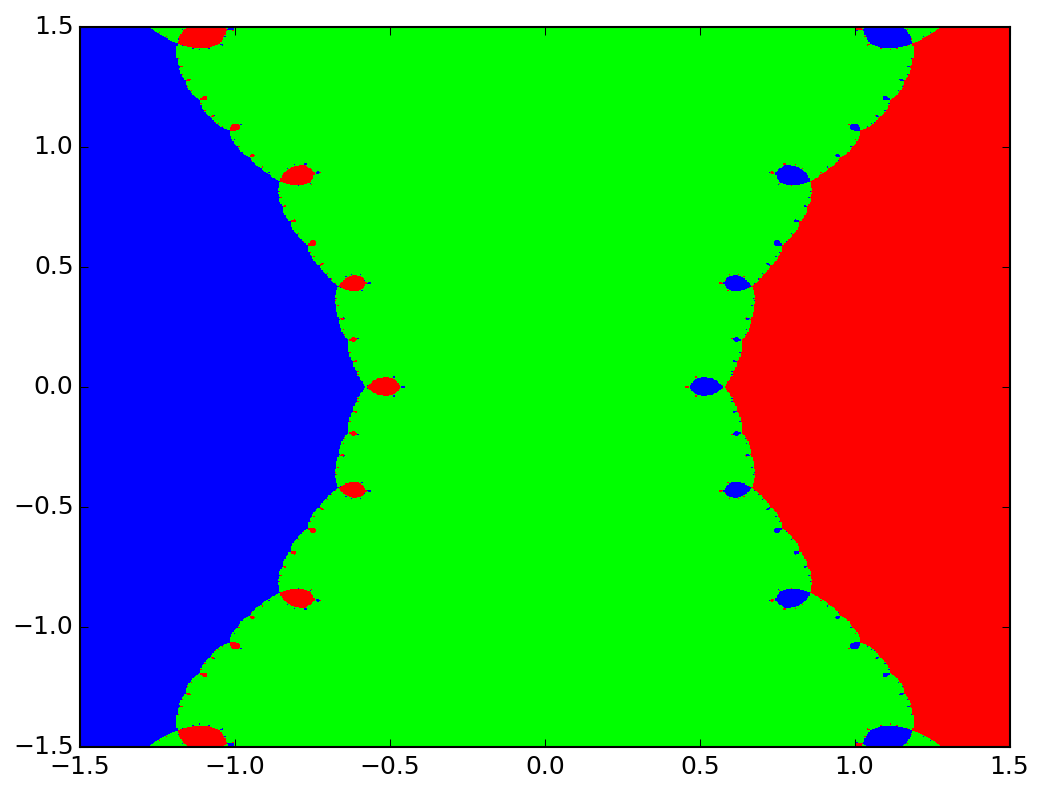
\includegraphics[width=\textwidth]{fractal_ex}
\end{subfigure}
\begin{subfigure}[b]{.49\textwidth}
\centering
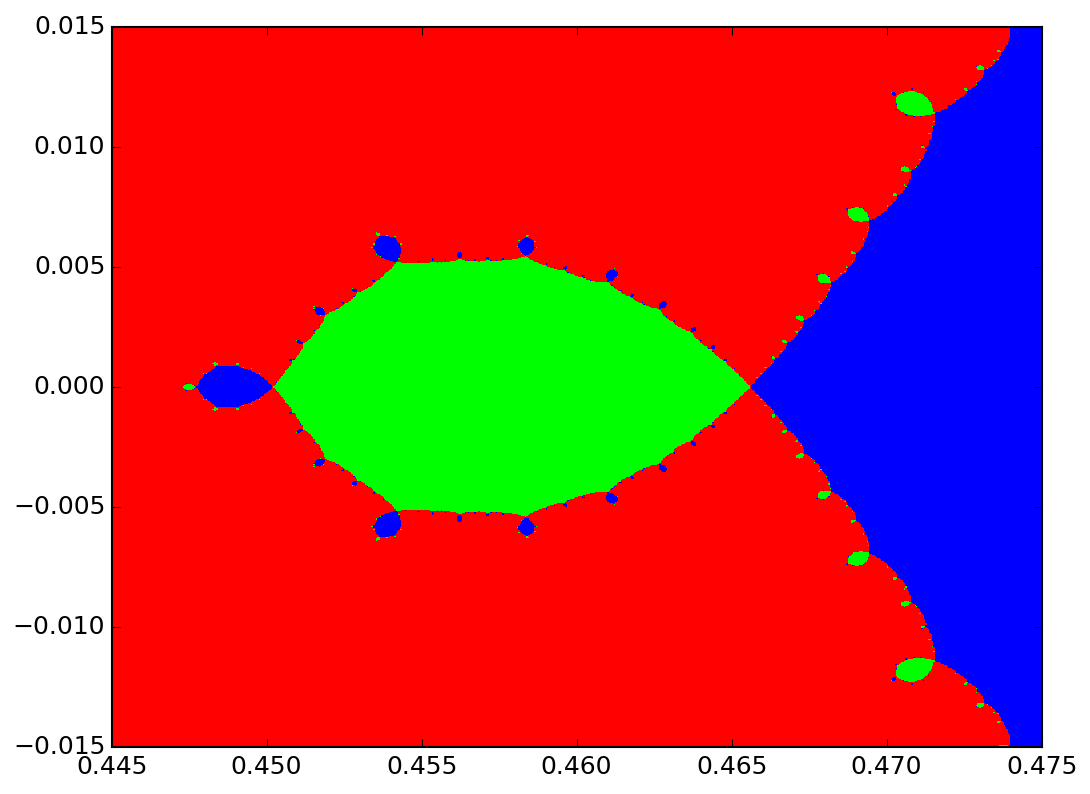
\includegraphics[width=\textwidth]{fractal_zoom}
\end{subfigure}
\caption{ Basins of attraction for $x^3-x$ in the complex plane. 
The picture on the right is a close-up of the figure on the left.}
\label{fig:fractal_ex}
\end{center}
\end{figure}

Newton fractals tell us that the long-term behavior of the Newton method is extremely sensitive to the initial guess $x_0$.
Changing $x_0$ by a small amount can change the output of Newton's method in a seemingly random way.
This is an example of \emph{chaos}.





\begin{problem}
\leavevmode
\begin{enumerate}
\item Complete the following function to plot the basins of attraction of a function.
\begin{lstlisting}
def plot_basins(f, Df, roots, xmin, xmax, ymin, ymax, numpoints=100, iters=15, colormap='brg'):
    '''Plot the basins of attraction of f.
    
    INPUTS:
    f       - A function handle. Should represent a function 
            from C to C.
    Df      - A function handle. Should be the derivative of f.
    roots   - An array of the zeros of f.
    xmin, xmax, ymin, ymax - Scalars that define the domain 
            for the plot.
    numpoints - A scalar that determines the resolution of 
            the plot. Defaults to 100.
    iters   - Number of times to iterate Newton's method. 
            Defaults to 15.
    colormap - A colormap to use in the plot. Defaults to 'brg'.    
    '''
\end{lstlisting}
You can test your function on the example $f(x) = x^3-x$ above. 

When the function \li{plt.pcolormesh()} is called on a complex array, it evaluates only on the real part of the complex numbers.
This means that if two roots of \li{f} have the same real part, their basins will be the same color if you plot directly using \li{plt.pcolormesh()}.

One way to fix this problem is to compute \li{Xnew} as usual.
Then iterate through the entries of \li{Xnew} and identify which root each entry is using the input \li{roots}.
Finally, create a new array whose entries are integers corresponding to these roots.
Plot the array of integers to view the basins of attraction.


\item Run \li{plot_basins()} on the function $x^3-1$ on the domain $\{a+bi \mid (a, b) \in [-1.5, 1.5] \times [-1.5, 1.5] \}$. 
The resulting plot should look like Figure \ref{fig:fractal_hw}.


\end{enumerate}
\begin{figure}[H]
\begin{center}
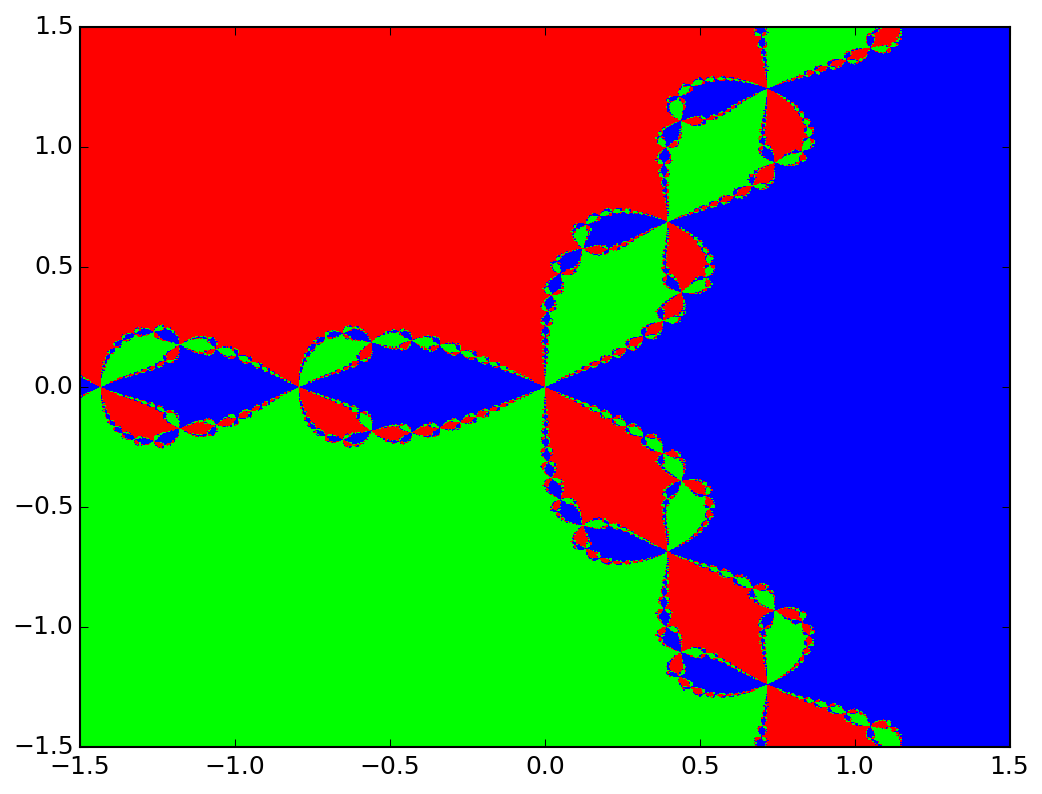
\includegraphics[scale=0.66]{fractal_hw}
\caption{Basins of attraction for $x^3-1$.}
\label{fig:fractal_hw}
\end{center}
\end{figure}
\end{problem}


% The remainder of the material has nothing to do with this lab, except that it mentions fractals.
\begin{comment}
Another well-studied fractal in the complex plane is the Mandelbrot set.
It is defined as the points $c \in \mathbb{C}$ for which the sequence
\[z_n = z_{n-1}^2 + c\]
is bounded.

\begin{problem}
Generate another grid of complex numbers on $[-1.5,.5]\times[-i,i]$.
Consider the recurrence relation $x_n = x_{n-1}^2 + c$.
Run this iteration 30 times with a resolution of $200 \times 200$ and display the plot.
\end{problem}
\end{comment}
